\documentclass[11pt,a4paper]{article}

%==============================================================
% PACKAGES
%==============================================================
% --- Encoding and language ---
\usepackage[utf8]{inputenc}
\usepackage[T1]{fontenc}
\usepackage{lmodern}
\usepackage[english]{babel}
\usepackage{microtype}
\usepackage{textgreek}
\usepackage{physics}
\newcommand{\dt}[1]{\dot{#1}}
\newcommand{\ddt}[1]{\ddot{#1}}

% --- Layout ---
\usepackage[margin=2.3cm,top=2.2cm,bottom=2.2cm]{geometry}
\setlength{\headheight}{14pt}
\usepackage{fancyhdr}
\usepackage{enumitem}
\usepackage{mdframed}      % caja gris para los enunciados de las preguntas
\usepackage{titlesec}
\titlespacing*{\section}{0pt}{1.2ex plus 0.2ex minus 0.1ex}{0.5ex plus 0.1ex minus 0.1ex}
\titlespacing*{\subsection}{0pt}{0.9ex plus 0.2ex minus 0.1ex}{0.3ex plus 0.1ex minus 0.1ex}

% --- Spacing around equations ---
\setlength{\abovedisplayskip}{5pt plus 1pt minus 1pt}
\setlength{\belowdisplayskip}{5pt plus 1pt minus 1pt}
\setlength{\abovedisplayshortskip}{2pt plus 1pt minus 1pt}
\setlength{\belowdisplayshortskip}{2pt plus 1pt minus 1pt}

% --- Mathematics and units ---
\usepackage{amsmath, amssymb, amsfonts}
\usepackage{bm}
\usepackage{siunitx}
\sisetup{per-mode=symbol}
\newcommand{\en}{\bm{e}_n}
\newcommand{\et}{\bm{e}_t}

% --- Figures and tables ---
\usepackage{graphicx}
\usepackage{epstopdf}      % permite incluir .eps (las figuras de Matlab se guardan como .eps)
\usepackage{xcolor}
\usepackage{caption}
\usepackage{subcaption}
\usepackage{booktabs}
\usepackage{float}
\usepackage{tikz}          % por si se quiere dibujar el esquema del carrete
\graphicspath{{figures/}{figs/}}

% --- Matlab code listings ---
\usepackage{listings}
\lstset{
  language=Matlab,
  basicstyle=\ttfamily\footnotesize,
  keywordstyle=\color{blue},
  commentstyle=\color{green!50!black},
  numbers=left,
  numberstyle=\tiny,
  frame=single,
  breaklines=true
}

% --- Links and cross-references (cargar al final) ---
\usepackage[hidelinks]{hyperref}
\usepackage[capitalise,noabbrev]{cleveref}

%==============================================================
% DOCUMENT DATA  (editar solo aqui)
%==============================================================
\newcommand{\labnumber}{1}
\newcommand{\labgroup}{LA}   % LA o LB

\title{Particle Connected to a Spool}
\author{Aimar Álvarez Iglesias \and
        Héctor Gonzalez Rodriguez \and
        Santiago Hernández Bejarano}
\date{\today}

%==============================================================
% STYLE
%==============================================================
% --- Header / footer ---
\pagestyle{fancy}
\fancyhf{}
\lhead{Mechanics Applied to Aerospace Engineering}
\rhead{Lab \labnumber{} -- Group \labgroup}
\cfoot{\thepage}
\renewcommand{\headrulewidth}{0.4pt}

% --- Abstract compacto (para que abstract + indice quepan en una pagina) ---
\renewenvironment{abstract}{%
  \begin{center}\bfseries\small\abstractname\end{center}%
  \vspace{-1em}\begin{quotation}\footnotesize}{%
  \end{quotation}\vspace{0.5em}}

% --- Los enunciados de las preguntas se escriben con el entorno estandar
%     "quote", que aqui se redefine como caja gris. Asi el Visual Editor de
%     Overleaf lo muestra como un bloque de cita normal. ---
\renewenvironment{quote}{%
  \par\medskip
  \begin{mdframed}[backgroundcolor=gray!12, hidealllines=true,
    innerleftmargin=8pt, innerrightmargin=8pt,
    innertopmargin=6pt, innerbottommargin=6pt]\small\itshape\emergencystretch=3em}{%
  \end{mdframed}\par\medskip}

% --- Portada: se redefine \maketitle (en el Visual Editor se vera el titulo
%     estandar, pero el PDF usa esta portada centrada) ---
\makeatletter
\renewcommand{\maketitle}{%
  \begin{titlepage}
    \centering
    \vspace*{0.2cm}

    \IfFileExists{logo_uc3m.png}{%
      
\includegraphics[width=0.30\textwidth]{logo_uc3m.png}\par
      \vspace{0.8cm}
    }{\vspace{1.5cm}}

    {\Large\bfseries Universidad Carlos III de Madrid\par}
    \vspace{0.25cm}
    {\large Aerospace Engineering\par}

    \vspace{1.2cm}

    \noindent\rule{\linewidth}{0.5pt}\par
    \vspace{0.4cm}
    {\huge\bfseries Computer Laboratory Report \labnumber\par}
    \vspace{0.35cm}
    {\LARGE \@title\par}
    \vspace{0.4cm}
    \noindent\rule{\linewidth}{0.5pt}\par

    \vspace{1.0cm}

    {\large Mechanics Applied to Aerospace Engineering\par}
    \vspace{0.25cm}
    {\large Laboratory Group \labgroup\par}

    \vspace{1.0cm}

    {\large\bfseries Authors\par}
    \vspace{0.3cm}
    {\large\def\and{\\}\renewcommand{\arraystretch}{1.3}%
     \begin{tabular}{c}\@author\end{tabular}\par}

    \vfill

    {\large \@date\par}
    \vspace*{0.2cm}
  \end{titlepage}}
\makeatother

%==============================================================
\begin{document}
%==============================================================

\maketitle

\tableofcontents
\newpage

%==============================================================
\section{Introduction}
In this experiment, we study the movement of a particle $P$ of mass $m$ connected by a thin, massless, inelastic, string of length $l$ that always remains in tension, to a cylindrical spool of radius $a$ centered in the origin of the coordinates $O$. The spool rotates at a constant angular velocity $\omega$ in a counterclockwise direction. The instantaneous tangential point between the string and the spool is called $B$ and the position is parameterized with the angle between the horizontal axis and the radius $OB$.

Our objective is to analyze the behavior of the particle in different cases of angular velocity and initial conditions, discussing the resulting dynamics, such as the tension in the string, energy conservation, and the trajectory of the particle. 

%==============================================================
\section{Methodology}\label{sec:method}
\subsection{Study of the Degrees of freedom}
\begin{figure}[htbp]
\centering
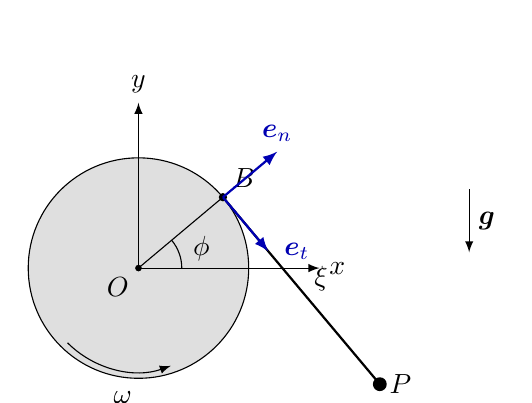
\begin{tikzpicture}[scale=1.0,>=latex]
\def\a{1.4}\def\ph{40}\def\xx{3.1}
\pgfmathsetmacro{\bx}{\a*cos(\ph)}\pgfmathsetmacro{\by}{\a*sin(\ph)}
\pgfmathsetmacro{\px}{\bx+\xx*sin(\ph)}\pgfmathsetmacro{\py}{\by-\xx*cos(\ph)}
\fill[gray!25] (0,0) circle (\a); \draw (0,0) circle (\a);
\draw[->] (0,0) -- (2.3,0) node[right] {$x$}; \draw[->] (0,0) -- (0,2.1) node[above] {$y$};
\fill (0,0) circle (1.2pt) node[below left] {$O$};
\draw (0,0) -- (\bx,\by);
\draw[thick] (\bx,\by) -- (\px,\py);
\fill (\bx,\by) circle (1.5pt) node[above right] {$B$};
\fill (\px,\py) circle (2.5pt) node[right] {$P$};
\draw[->,thick,blue!70!black] (\bx,\by) -- ++({0.9*cos(\ph)},{0.9*sin(\ph)}) node[above] {$\en$};
\draw[->,thick,blue!70!black] (\bx,\by) -- ++({0.9*sin(\ph)},{-0.9*cos(\ph)}) node[right,xshift=2pt] {$\et$};
\draw (0.55,0) arc (0:\ph:0.55); \node at (0.8,0.25) {$\phi$};
\node at ({(\bx+\px)/2+0.25},{(\by+\py)/2+0.15}) {$\xi$};
\draw[->] (4.2,1.0) -- (4.2,0.2) node[midway,right] {$\bm g$};
\draw[->] (-0.9,-0.95) arc (225:290:1.25); \node at (-0.2,-1.65) {$\omega$};
\end{tikzpicture}
\caption{Geometry of the problem and local basis $\{\en,\et\}$ attached to the point of tangency $B$.}\label{fig:geom}
\end{figure}
Let $\en=(\cos\phi,\sin\phi)$ be the unit vector along $OB$ and $\et=(\sin\phi,-\cos\phi)$ the unit vector tangent to the spool
at $B$, oriented along the free segment from $B$ to $P$ (Fig.~\ref{fig:geom}). Since $\dt{\phi}$ is the rotation rate of both
vectors,
\begin{equation}
\dt{\bm e}_n=-\dt{\phi}\,\et,\qquad \dt{\bm e}_t=\dt{\phi}\,\en .
\label{eq:basis}
\end{equation}
\textbf{Degrees of freedom.} The particle $P$ is free on a plane, so it has two coordinates to move along. The string attached to the particle imposes a constraint: the sum between length of the wound arc (let the attachment point be $A$) $AB$ and the length of the segment $BP$ must equal $l$, and $l = AB + BP = \text{constant}$. The point of tangency can vary, but the total length of the string cannot. Hence, $2-1=1$ configuration degree of freedom, which can be parametrised with $\phi$.
If $\alpha(t)=\alpha_0+\omega t$ is the angular position of the attachment point on the spool, the arc wound on the spool (clockwise from the attachment point to $B$) is $a[\alpha(t)-\phi]$, where $[\alpha(t)-\phi]$ is the angular difference between the attachment point and $B$, and the inextensibility $l=a[\alpha(t)-\phi]+\xi$, where $\xi$ is the variable length of the segment $BP$, gives, using $\xi(0)=\xi_0$ and $\phi(0)=0$,
\begin{equation}
\xi(t,\phi)=\xi_0+a\,\phi-a\,\omega\,t .
\label{eq:xi}
\end{equation}
Therefore the position of $P$,
\begin{equation}
\bm r_P=a\,\en+\xi\,\et=\begin{pmatrix}a\cos\phi+\xi\sin\phi\\ a\sin\phi-\xi\cos\phi\end{pmatrix},
\label{eq:pos}
\end{equation}
is completely determined by $\phi$ and $t$: the system has \textbf{one configuration degree of freedom}, parametrised by $\phi$.
Geometrically, $P$ lies on the involute of the spool circle; for $\omega\neq0$ the involute rotates rigidly with the spool
(its starting angle is $\omega t-\xi_0/a$), so the constraint depends explicitly on time. For $\omega=0$ the constraint is
time independent.

\textbf{Velocity and acceleration.} Using Eq.~\eqref{eq:basis} and $\dt{\xi}=a(\dt{\phi}-\omega)$,
\begin{align}
\bm v_P&=(\dt{\xi}-a\dt{\phi})\,\et+\xi\dt{\phi}\,\en=\xi\dt{\phi}\,\en-a\omega\,\et ,\label{eq:vel}\\
\bm a_P&=\big(\xi\ddt{\phi}+a\dt{\phi}^{2}-2a\omega\dt{\phi}\big)\,\en-\xi\dt{\phi}^{2}\,\et .\label{eq:acc}
\end{align}
Equation~\eqref{eq:vel} shows that the velocity component along the string is fixed by the spool, $\bm v_P\cdot\et=-a\omega$ (the
string cannot stretch), and that the component normal to the string is $\xi\dt{\phi}$. The initial condition therefore satisfies
$\dt{x}_P(0)=\xi_0\dt{\phi}(0)$, i.e.\ $\dt{\phi}(0)=\dt{x}_P(0)/\xi_0$, while $\dt{y}_P(0)=a\omega$ is not free but imposed by the constraint.

\subsection{Forces and equation of motion}
Only two forces act on $P$: its weight and the tension $T$ of the string, which pulls $P$ towards $B$:
\begin{equation}
\bm F=-mg\,\bm j-T\,\et,\qquad T\geq0,\qquad -mg\,\bm j=mg\cos\phi\,\et-mg\sin\phi\,\en .
\label{eq:forces}
\end{equation}
Writing Newton's second law $m\bm a_P=\bm F$ in the directions $\en$ and $\et$:
\begin{align}
\xi\ddot{\phi}+a\dt{\phi}^{2}-2a\omega\dt{\phi}&=-g\sin\phi ,\label{eq:eomn}\\
T&=m\big(g\cos\phi+\xi\dt{\phi}^{2}\big).\label{eq:T}
\end{align}
The tension does not appear in the first equation, because it has no component along $\en$. So the first equation alone gives the motion:
\begin{equation}
\ddot{\phi}=-\frac{g\sin\phi+a\dt{\phi}^{2}-2a\omega\dt{\phi}}{\xi_0+a\phi-a\omega t},
\label{eq:eom}
\end{equation}
and once $\phi$ and $\dt\phi$ are known, Eq.~\eqref{eq:T} gives the tension. We can understand Eq.~\eqref{eq:eom} like this:
\begin{itemize}[noitemsep,topsep=2pt]
\item If the spool were very thin ($a\to0$), we would get a normal pendulum of length $\xi_0$: $\ddt\phi=-(g/\xi_0)\sin\phi$.
\item With $a>0$ the length of the pendulum changes while it swings, and this gives the term $a\dt\phi^2$.
\item The term $-2a\omega\dt\phi$ only exists if the spool turns.
\item When $\xi\to0$ (all the string is wrapped) we divide by zero: the particle hits the spool and the model is no longer valid.
\end{itemize}
Two simple results follow. First, if $\phi(0)=0$ and $\dt\phi(0)=0$, the right side of Eq.~\eqref{eq:eom} is zero and $\phi$ stays at zero: the particle just hangs down. Second, a string can pull but not push, so we need $T\geq0$, i.e.\ $\xi\dt\phi^2\geq-g\cos\phi$. This can only fail if $\cos\phi<0$, which means the string points above the horizontal line through $B$, and the particle moves slowly.

\subsection{Mechanical energy}

From Eqs.~\eqref{eq:pos} and \eqref{eq:vel}, with $|\bm v_P|^2=\xi^2\dt\phi^2+a^2\omega^2$ and $y_P=a\sin\phi-\xi\cos\phi$,
\begin{equation}
E=\tfrac12 m\left(\xi^{2}\dt{\phi}^{2}+a^{2}\omega^{2}\right)+mg\left(a\sin\phi-\xi\cos\phi\right).
\label{eq:E}
\end{equation}
Weight is conservative and is included in $E$, so $\dt E$ equals the power of the tension, $-T\et\cdot\bm v_P$, that is
\begin{equation}
\frac{dE}{d t}=a\,\omega\,T .
\label{eq:Edot}
\end{equation}
If $\omega=0$ the tension is perpendicular to the velocity, it does no work and $E$ stays constant. If $\omega>0$ the spool pulls the string, the tension does positive work and $E$ grows all the time while the string is tight.

\clearpage

\section{Results}\label{sec:results}
Figure~\ref{fig:state} shows $\phi$, $\xi$ and $T$ for each case, Fig.~\ref{fig:traj} the trajectories and Fig.~\ref{fig:energy} the energy.

\subsection{Case 1: rotating spool, particle starts at rest}
In Case 1, the particle is released from rest in the vertical downward position ($\phi(0)=0$, $\dt\phi(0)=0$). In the absence of lateral excitation, no angular oscillation is initiated, and the angle remains identically zero ($\phi(t)=0$). The spool rotates at constant rate, winding the string at the linear speed $a\omega = \SI{0.02}{m/s}$. Consequently, the unwound length decreases linearly as $\xi(t) = 1 - 0.02\,t$ (Fig.~\ref{fig:state}, top row). Because the vertical ascent occurs at constant velocity, the acceleration is zero, and the string tension equals the gravitational weight: $T = mg = \SI{0.981}{N}$. At $t = \xi_0/(a\omega) = \SI{50}{s}$, the entire 1-meter string is wound, and the particle contacts the spool surface. Because the particle velocity matches the tangential velocity of the spool at contact, no impulsive impact occurs. The mechanical energy increases linearly at the rate $a\omega mg = \SI{19.6}{mW}$ (Fig.~\ref{fig:energy}a), with a total energy gain of $mg\xi_0 = \SI{0.981}{J}$ corresponding to the gravitational potential energy gained over \SI{1}{m}.

\subsection{Case 2: fixed spool, small initial velocity}
In Case 2, the spool remains stationary ($\omega = 0$), and an initial horizontal velocity of $\SI{-1}{m/s}$ is applied to the left. The particle exhibits pendulum-like oscillations with variable string length. The motion displays geometric asymmetry: when the particle swings to the left ($\phi < 0$), string wraps onto the spool cylinder and the effective length decreases to a minimum of $\SI{0.934}{m}$; when it swings to the right ($\phi > 0$), string unwinds and extends to $\SI{1.063}{m}$. The angular range extends between $-18.8^\circ$ and $+18.0^\circ$. The oscillation period is $\SI{2.018}{s}$, slightly longer than the $\SI{2.006}{s}$ period of a standard 1-meter simple pendulum. The tension reaches a maximum of $T = \SI{1.08}{N}$ at the lowest point where the velocity peaks, and decreases to $\SI{0.93}{N}$ at the turning points where $\dt\phi=0$. The tension remains strictly positive, preventing string slackening throughout the 20-second simulation.

\clearpage
\begin{figure}[t]
\centering
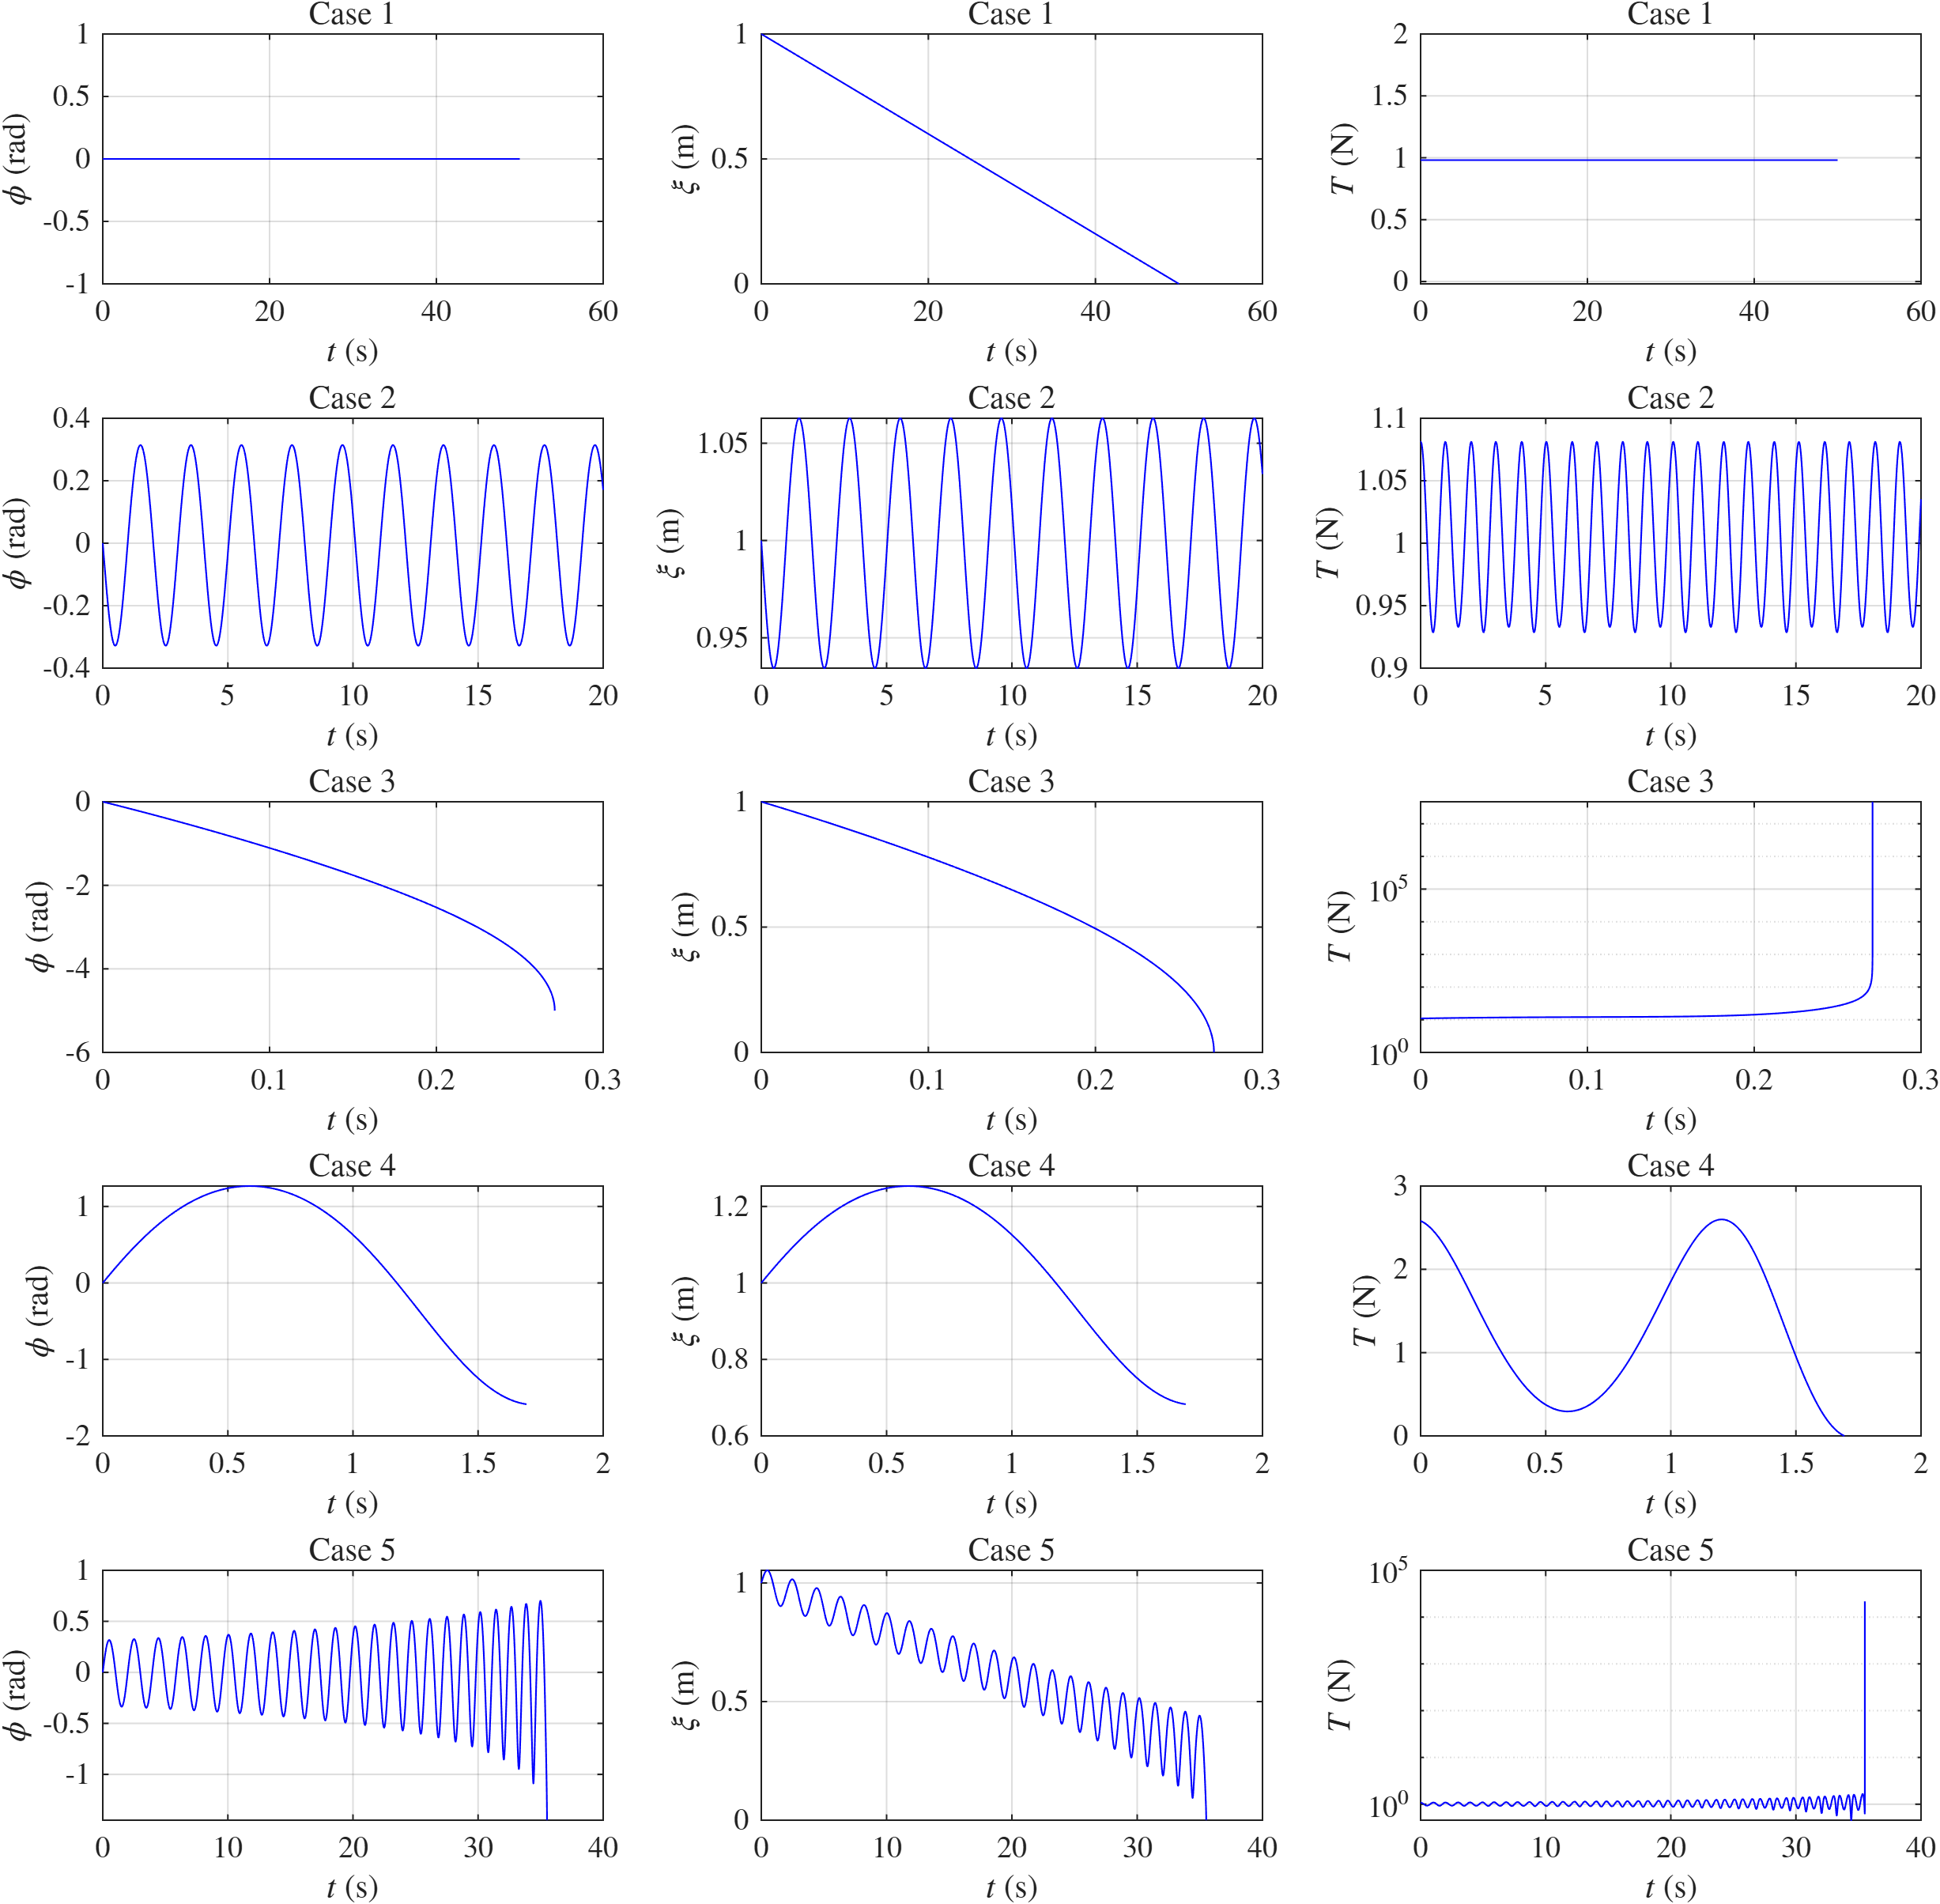
\includegraphics[width=0.54\textwidth]{Fig_1.png}
\caption{Angle $\phi$, free length $\xi$ and tension $T$ against time for the five cases (one case per row). In Cases 3 and 5 the tension is plotted in logarithmic scale because it becomes very large at the end.}\label{fig:state}
\end{figure}

\subsection{Case 3: fixed spool, large initial velocity}
In Case 3, a large initial velocity of $\SI{-10}{m/s}$ is applied to the left with $\omega=0$. The particle wraps around the spool in a rapid inward spiral. The unwound length reaches zero at $\phi = -\xi_0/a = -5\text{ rad}$ (approximately $0.8$ turns). Contact occurs at $t_f = \SI{0.2709}{s}$ at coordinates $(0.057,\,0.192)\text{ m}$ on the upper surface of the spool (Fig.~\ref{fig:traj}).

Near the contact point, the linear speed of the particle remains bounded at $v_s = \SI{8.75}{m/s}$ by energy conservation. However, because the instantaneous radius of curvature $\xi$ approaches zero, the angular velocity must diverge to preserve linear velocity: $|\dt\phi| \approx v_s/\xi$. The required centripetal force causes the string tension to escalate rapidly according to:
\begin{equation}
\dt\phi \simeq -\sqrt{\frac{v_s}{2a(t_f-t)}}, \qquad T \simeq \frac{m v_s^2}{\xi}.
\end{equation}
Both $\dt\phi$ and $T$ exhibit power-law divergence proportional to $(t_f - t)^{-1/2}$, confirmed by the $-1/2$ slope on the logarithmic scale in Figure~\ref{fig:extra}a. At $t = t_f$, the geometric singularity terminates the validity of the involute model upon physical impact.

\subsection{Case 4: fixed spool, loss of tension}
In Case 4, an initial positive velocity of $\SI{4}{m/s}$ is applied to the right with $\omega=0$. The particle ascends to $\phi = 72.6^\circ$ ($1.267\text{ rad}$) at $t = \SI{0.588}{s}$, where it halts and reverses direction. Accelerating through the bottom position, it climbs along the left side, wrapping onto the spool. Once the angle passes horizontal ($\phi < -90^\circ$), the unit vector $\et$ points upward, meaning the gravitational component along the string acts inward toward the spool center. To maintain tension, the centripetal acceleration must satisfy $\xi\dt\phi^2 \geq -g\cos\phi$. At $t = \SI{1.693}{s}$, the linear speed drops to $\SI{0.318}{m/s}$, and the tension vanishes at $\phi = -90.9^\circ$ and $\xi = \SI{0.683}{m}$ (Fig.~\ref{fig:state}, fourth row). The string becomes slack, violating the tensile constraint. Beyond this point, the particle transitions into unconstrained ballistic flight under gravity. Mechanical energy is strictly conserved at $E = \SI{-0.181}{J}$ up to the slackening event.

\clearpage
\begin{figure}[t]
\centering
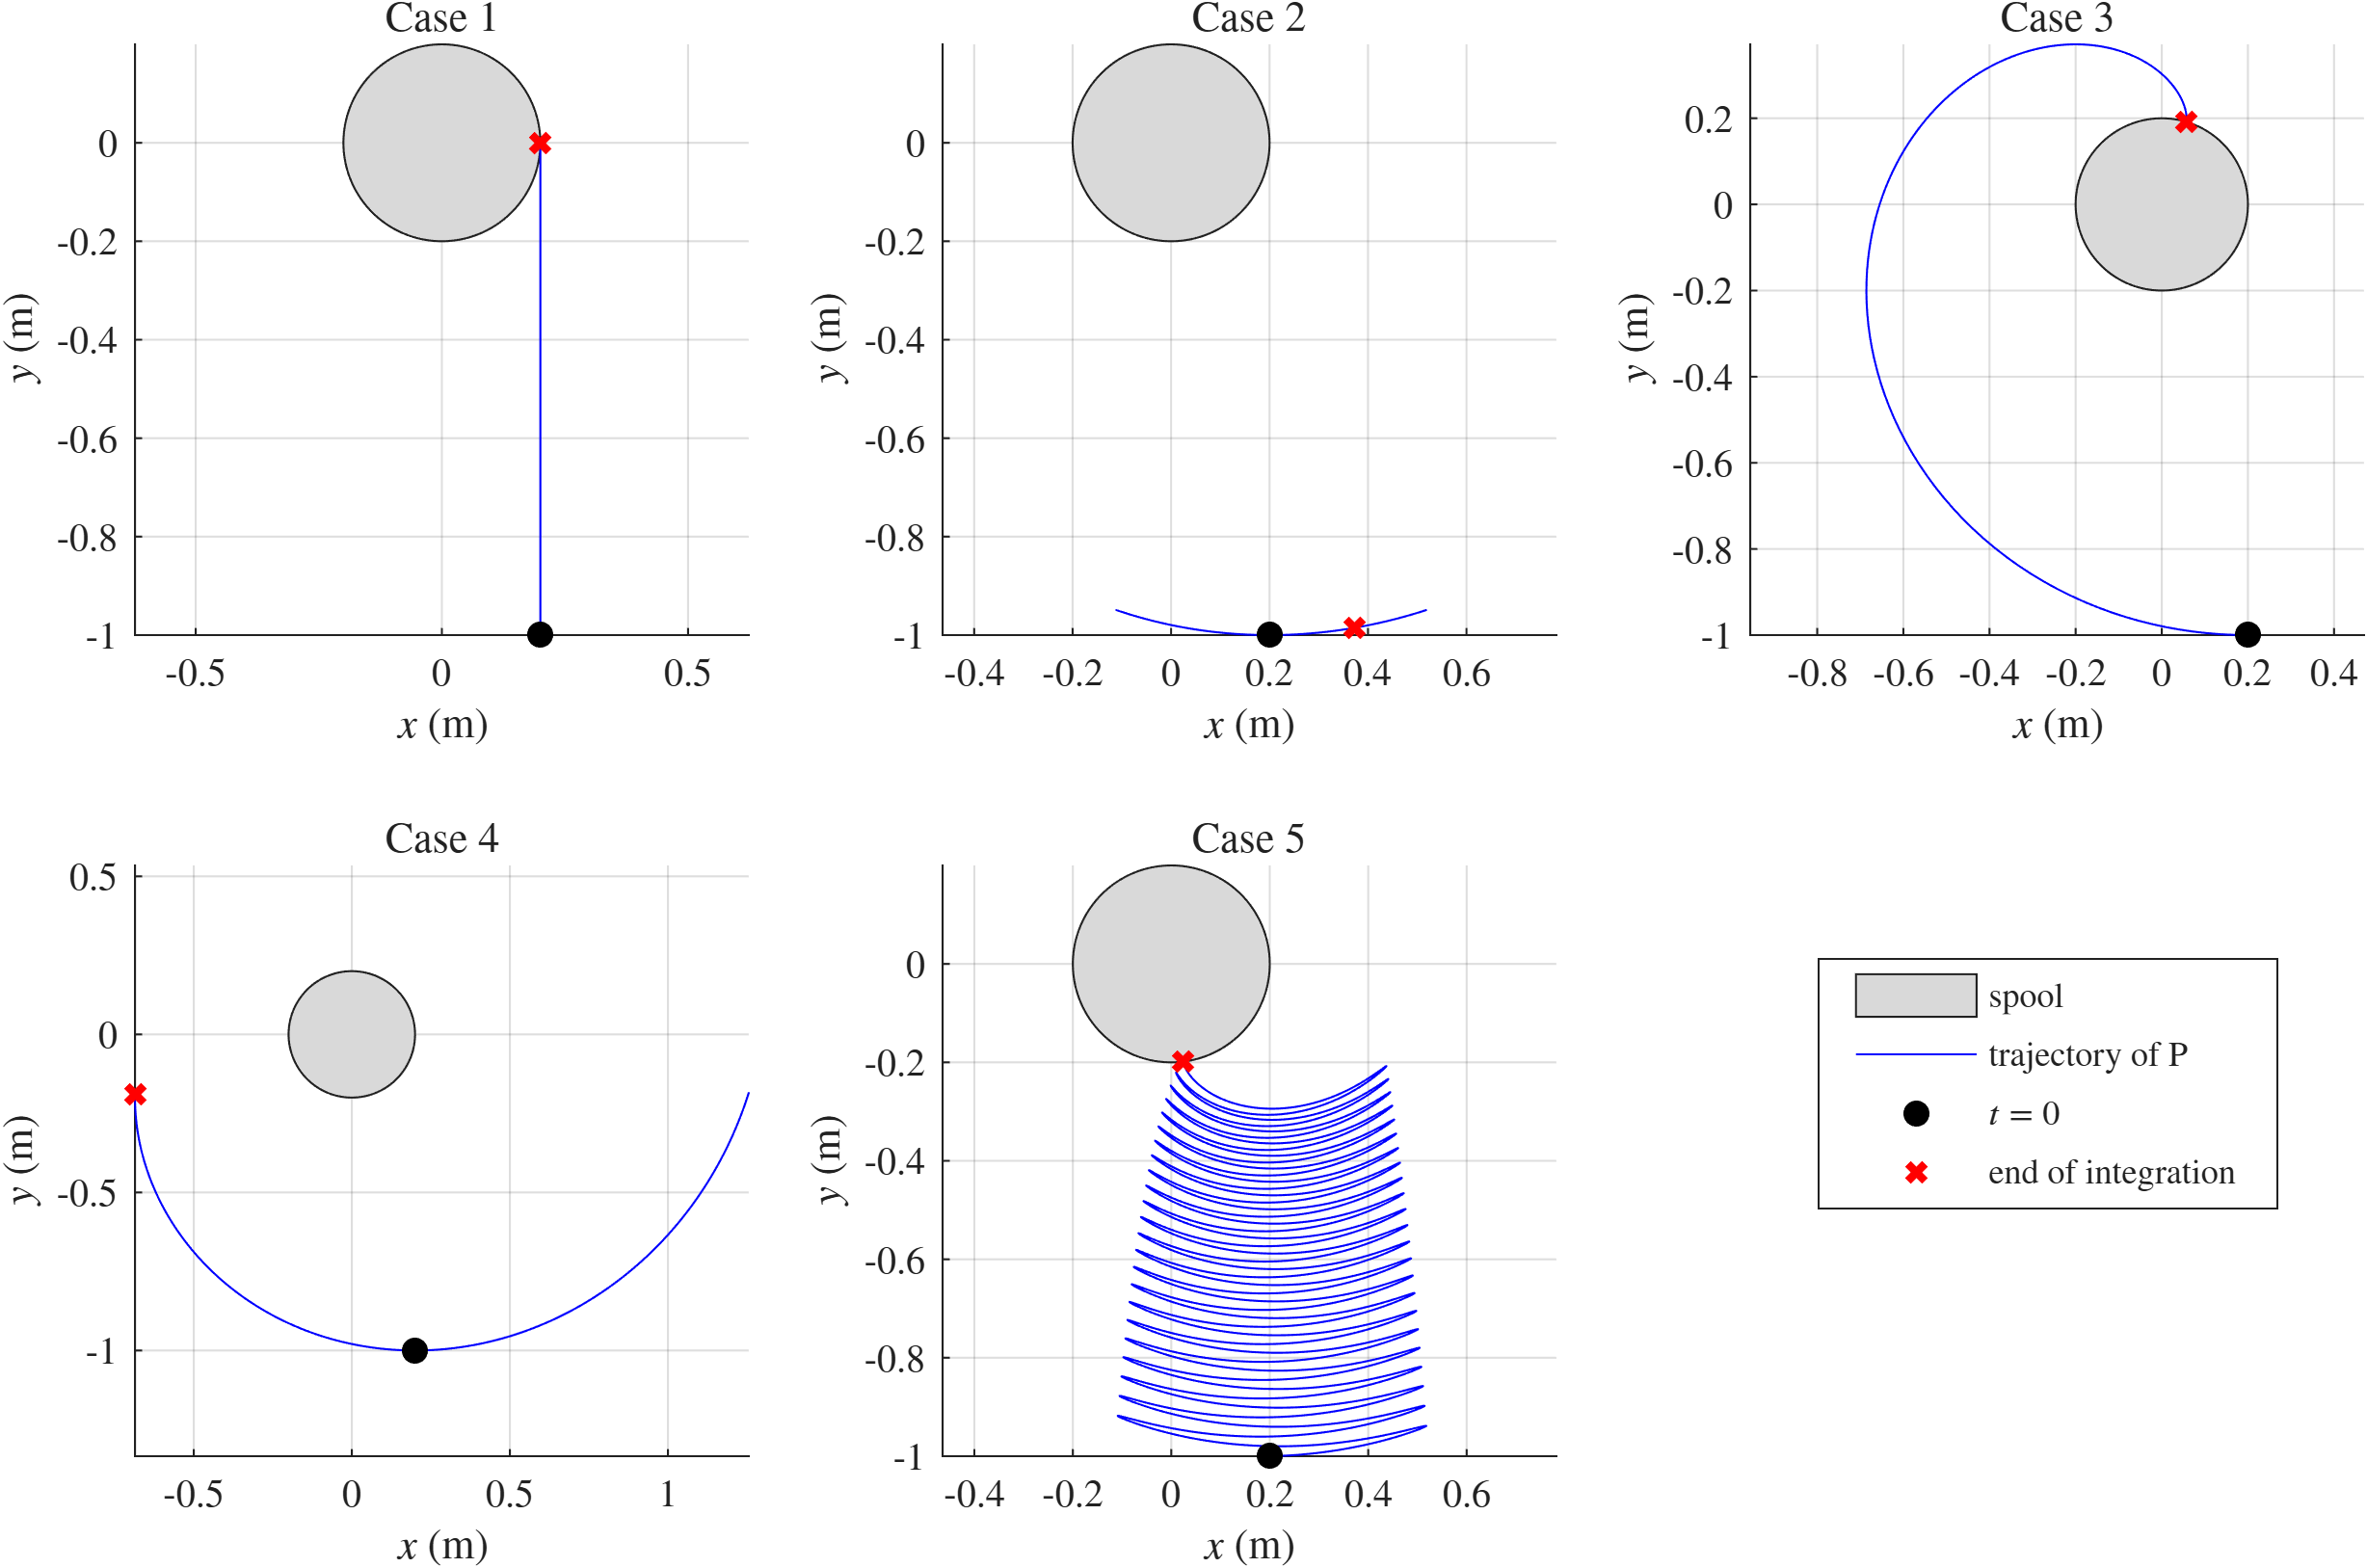
\includegraphics[width=0.70\textwidth]{Fig_2.png}
\caption{Trajectory of $P$ in the $Oxy$ plane for each case. The grey circle is the spool (drawn at $t=0$). The black dot is the start and the red cross the end of the integration.}\label{fig:traj}
\end{figure}

\subsection{Case 5: rotating spool with initial velocity}
In Case 5, the spool rotates at $\omega = \SI{0.1}{rad/s}$ while an initial velocity of $\SI{1}{m/s}$ is applied to the particle. On average, the unwound length decreases at the linear rate of $a\omega = \SI{0.02}{m/s}$. As the string shortens, the oscillation frequency increases, reducing the period from $\SI{2.0}{s}$ initially to $\SI{1.15}{s}$ near termination. Concurrently, the oscillation amplitude grows from $\pm 0.3\text{ rad}$ to $[-1.45,\, 0.70]\text{ rad}$ because the rotating spool performs net positive work on the particle during each cycle. The tension remains positive throughout (minimum $\SI{0.46}{N}$), preventing slackening. At $t = \SI{35.51}{s}$, the unwound length vanishes ($\xi = 0$), and the particle impacts the lower surface of the spool at $(0.024,\,-0.199)\text{ m}$ (Fig.~\ref{fig:traj}), accompanied by asymptotic escalation of $\dt\phi$ and $T$ as in Case 3.

\subsection{Energy}
The mechanical energy histories provide clear validation of the governing dynamics. For all unforced cases with $\omega = 0$ (Cases 2, 3, and 4), the string tension is everywhere orthogonal to the velocity vector, performing zero work. Mechanical energy is rigorously conserved (Fig.~\ref{fig:energy}b--d). Numerical drift remains below $10^{-9}$ in relative error (Fig.~\ref{fig:energy}f), confirming the accuracy of the integration scheme. When the spool rotates ($\omega = 0.1\text{ rad/s}$), the boundary condition performs work on the system at the rate $\dd E/\dd t = a\omega T$. In Case 1, the constant tension produces linear energy growth. In Case 5, tension oscillations induce cyclic fluctuations superimposed on an overall energy gain of $\SI{0.74}{J}$. Simultaneous integration of the external work $W(t) = \int_0^t a\omega T\,\dd t$ with \texttt{ode45} demonstrates exact agreement between $E(t) - E_0$ and $W(t)$ (Fig.~\ref{fig:extra}b), with residuals below $10^{-8}\text{ J}$.

\clearpage
\begin{figure}[t]
\centering
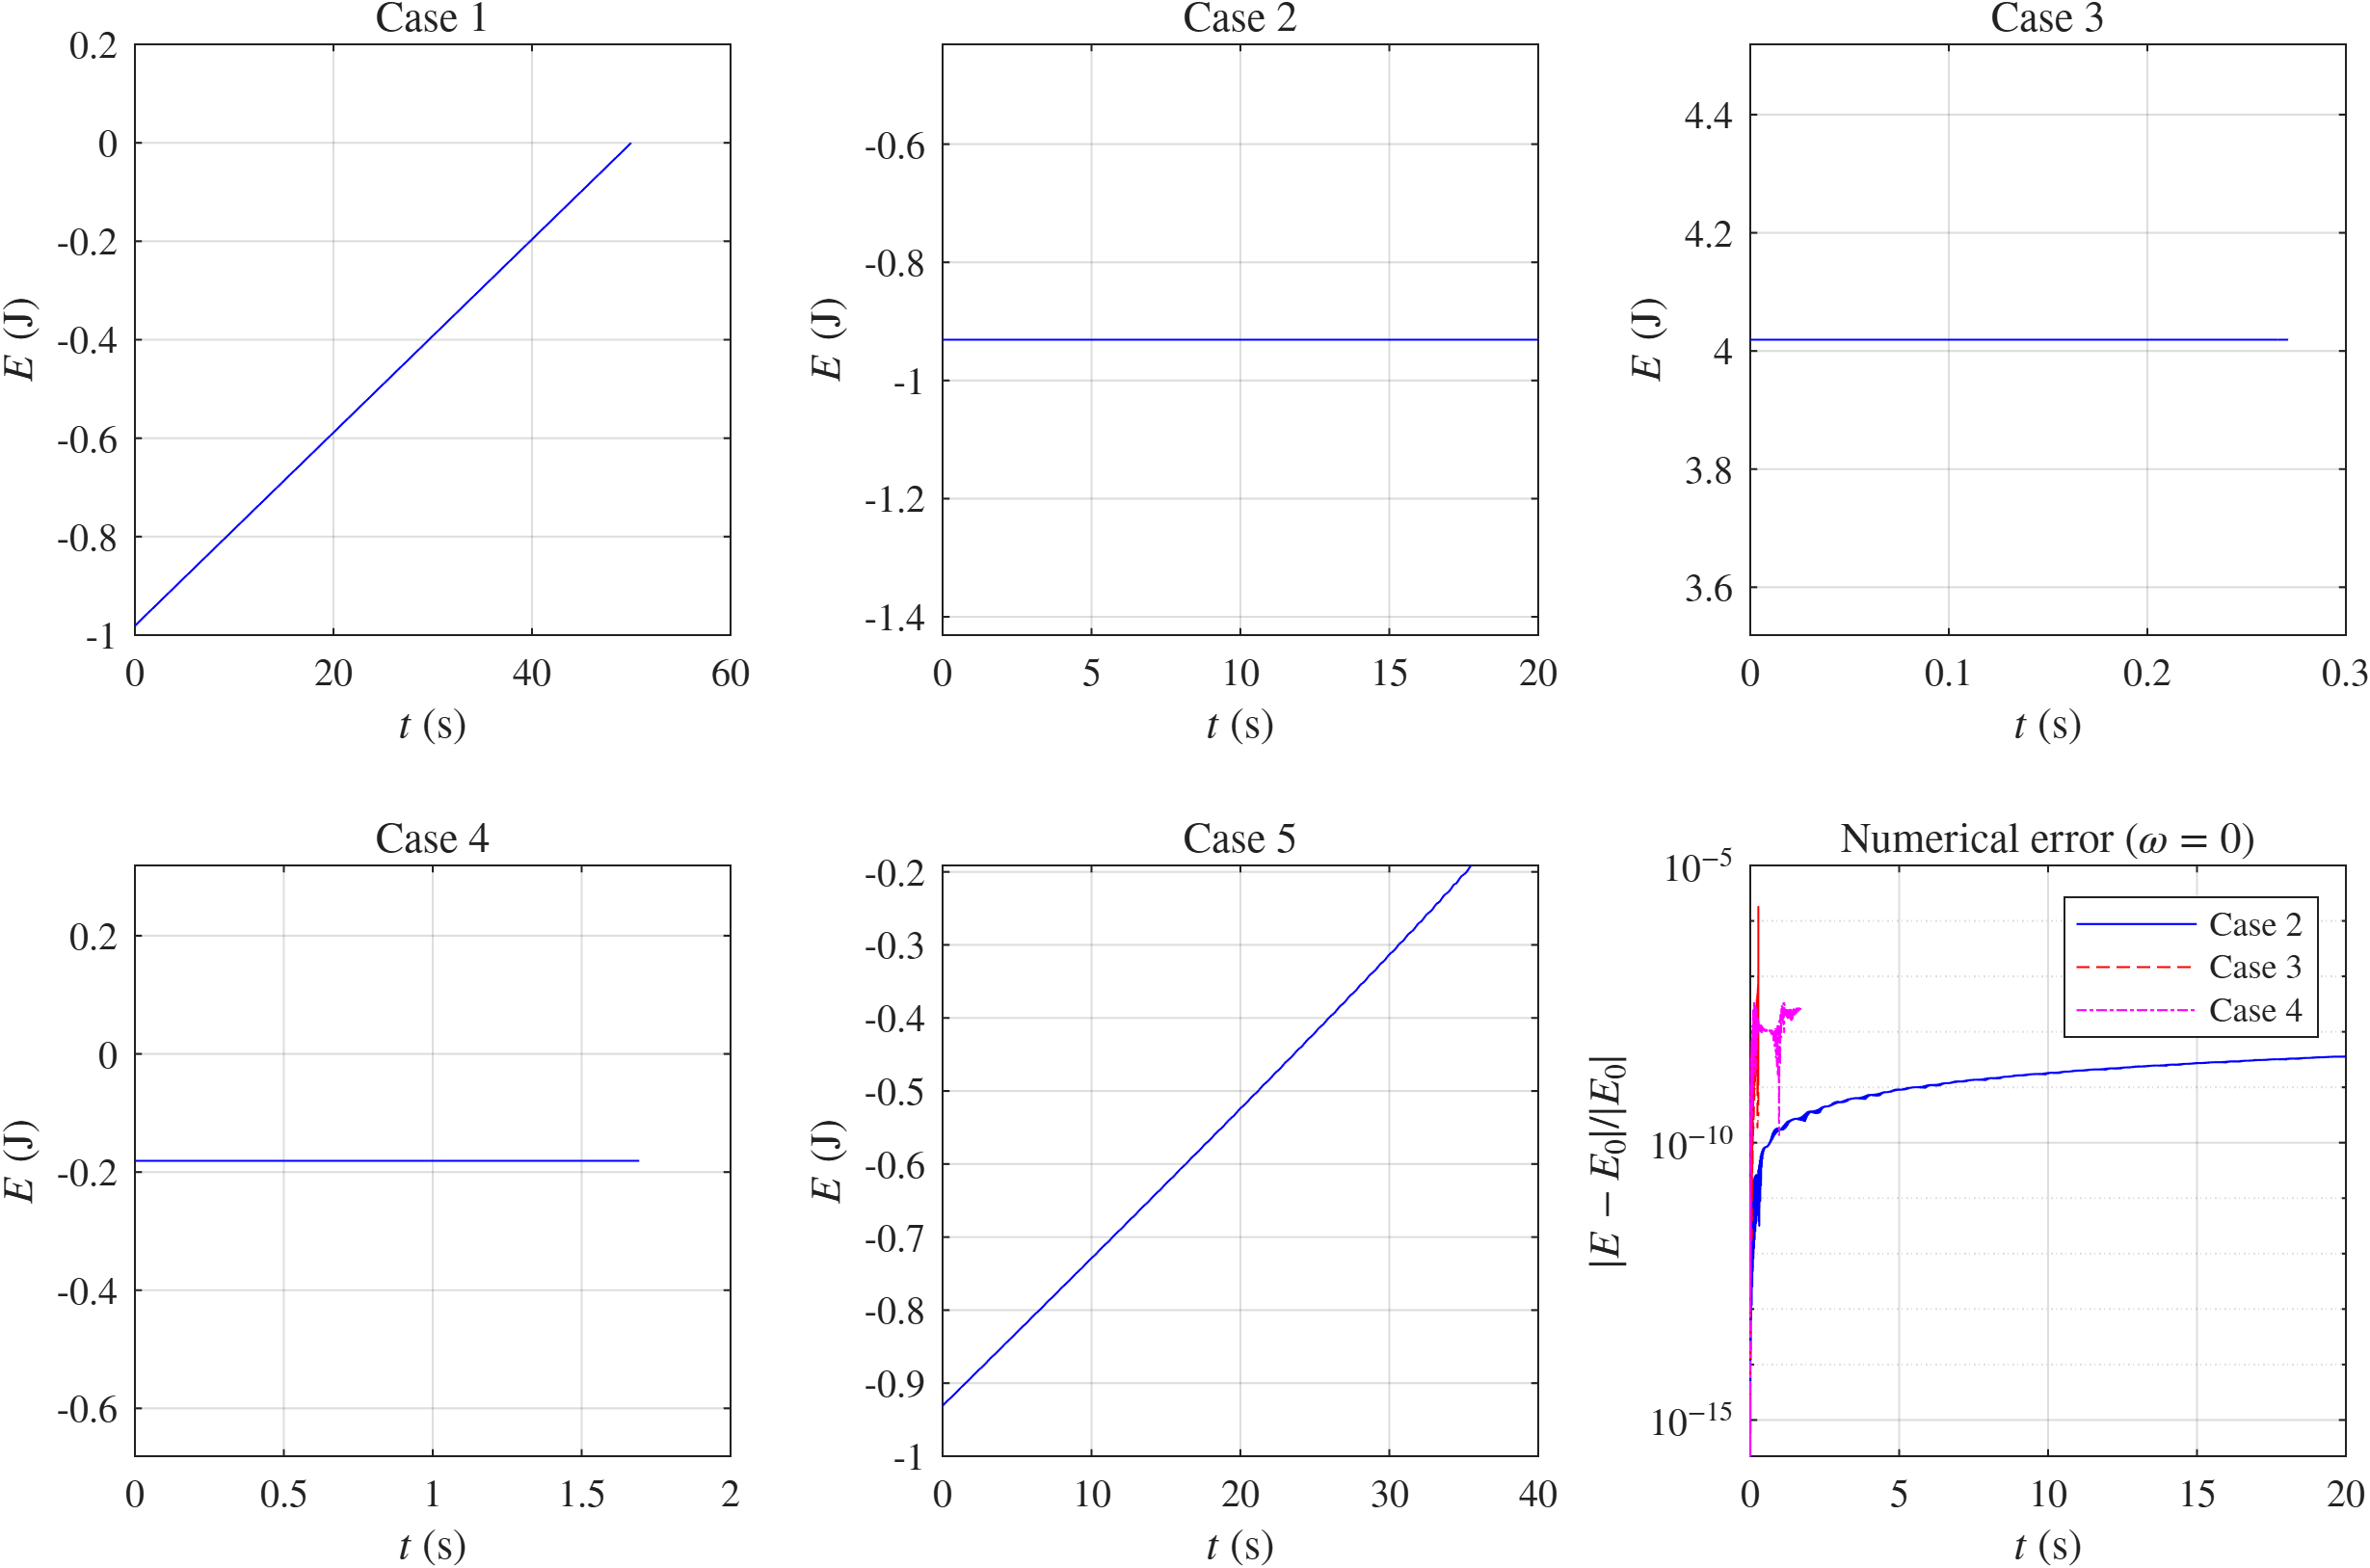
\includegraphics[width=0.70\textwidth]{Fig_3.png}
\caption{(a--e) Mechanical energy $E$ against time in Cases 1--5. For $\omega=0$ the vertical axis covers $\pm0.5$ J around $E_0$. (f) Relative change of the energy for the cases with $\omega=0$.}\label{fig:energy}
\end{figure}


\section{Discussion: motion after the string becomes loose}\label{sec:discussion}
In Case 4 the integration stops when $T=0$. After that moment the string is loose, so Eq.~\eqref{eq:eom} is not valid anymore: the particle is free and moves only under gravity, with two degrees of freedom. To continue the simulation, the code could be changed like this (always using \texttt{ode45}):
\begin{enumerate}[noitemsep,topsep=2pt]
\item Take the values at the event ($t^*$, $\phi^*$, $\dt\phi^*$) and calculate the position and velocity of $P$ in $x$ and $y$ with Eqs.~\eqref{eq:pos} and \eqref{eq:vel}. The new state is $\bm X_2=[x,y,\dt x,\dt y]^T$.
\item Write the free fall, $\ddt x=0$, $\ddt y=-g$, as a first order system for $\bm X_2$ and integrate it with \texttt{ode45} from $t^*$.
\item Use a new event function with two events: (i) the string becomes tight again, which happens when the wrapped part plus the straight part is equal to $l$; (ii) the particle hits the spool, $\sqrt{x^2+y^2}=a$.
\item When the string becomes tight again, it pulls the particle suddenly. The part of the velocity along the string is changed so that it is again $-a\omega$ (Eq.~\eqref{eq:vel}), and only the part perpendicular to the string stays. This is like an inelastic collision, so some kinetic energy is lost at that moment. With the new velocity we calculate $\phi$ and $\dt\phi$ and continue with Eq.~\eqref{eq:eom} and \texttt{ode45}.
\item Put everything inside a loop that changes between the "tight" and the "loose" parts until the particle hits the spool or the final time is reached, and join all the parts to make the plots.
\end{enumerate}
In Case 4 the speed at the event is only $\SI{0.32}{m/s}$ and almost vertical, so the particle would make a short free flight and then the string would become tight again, with a small loss of energy.


\clearpage

\begin{figure}[htbp]
\centering
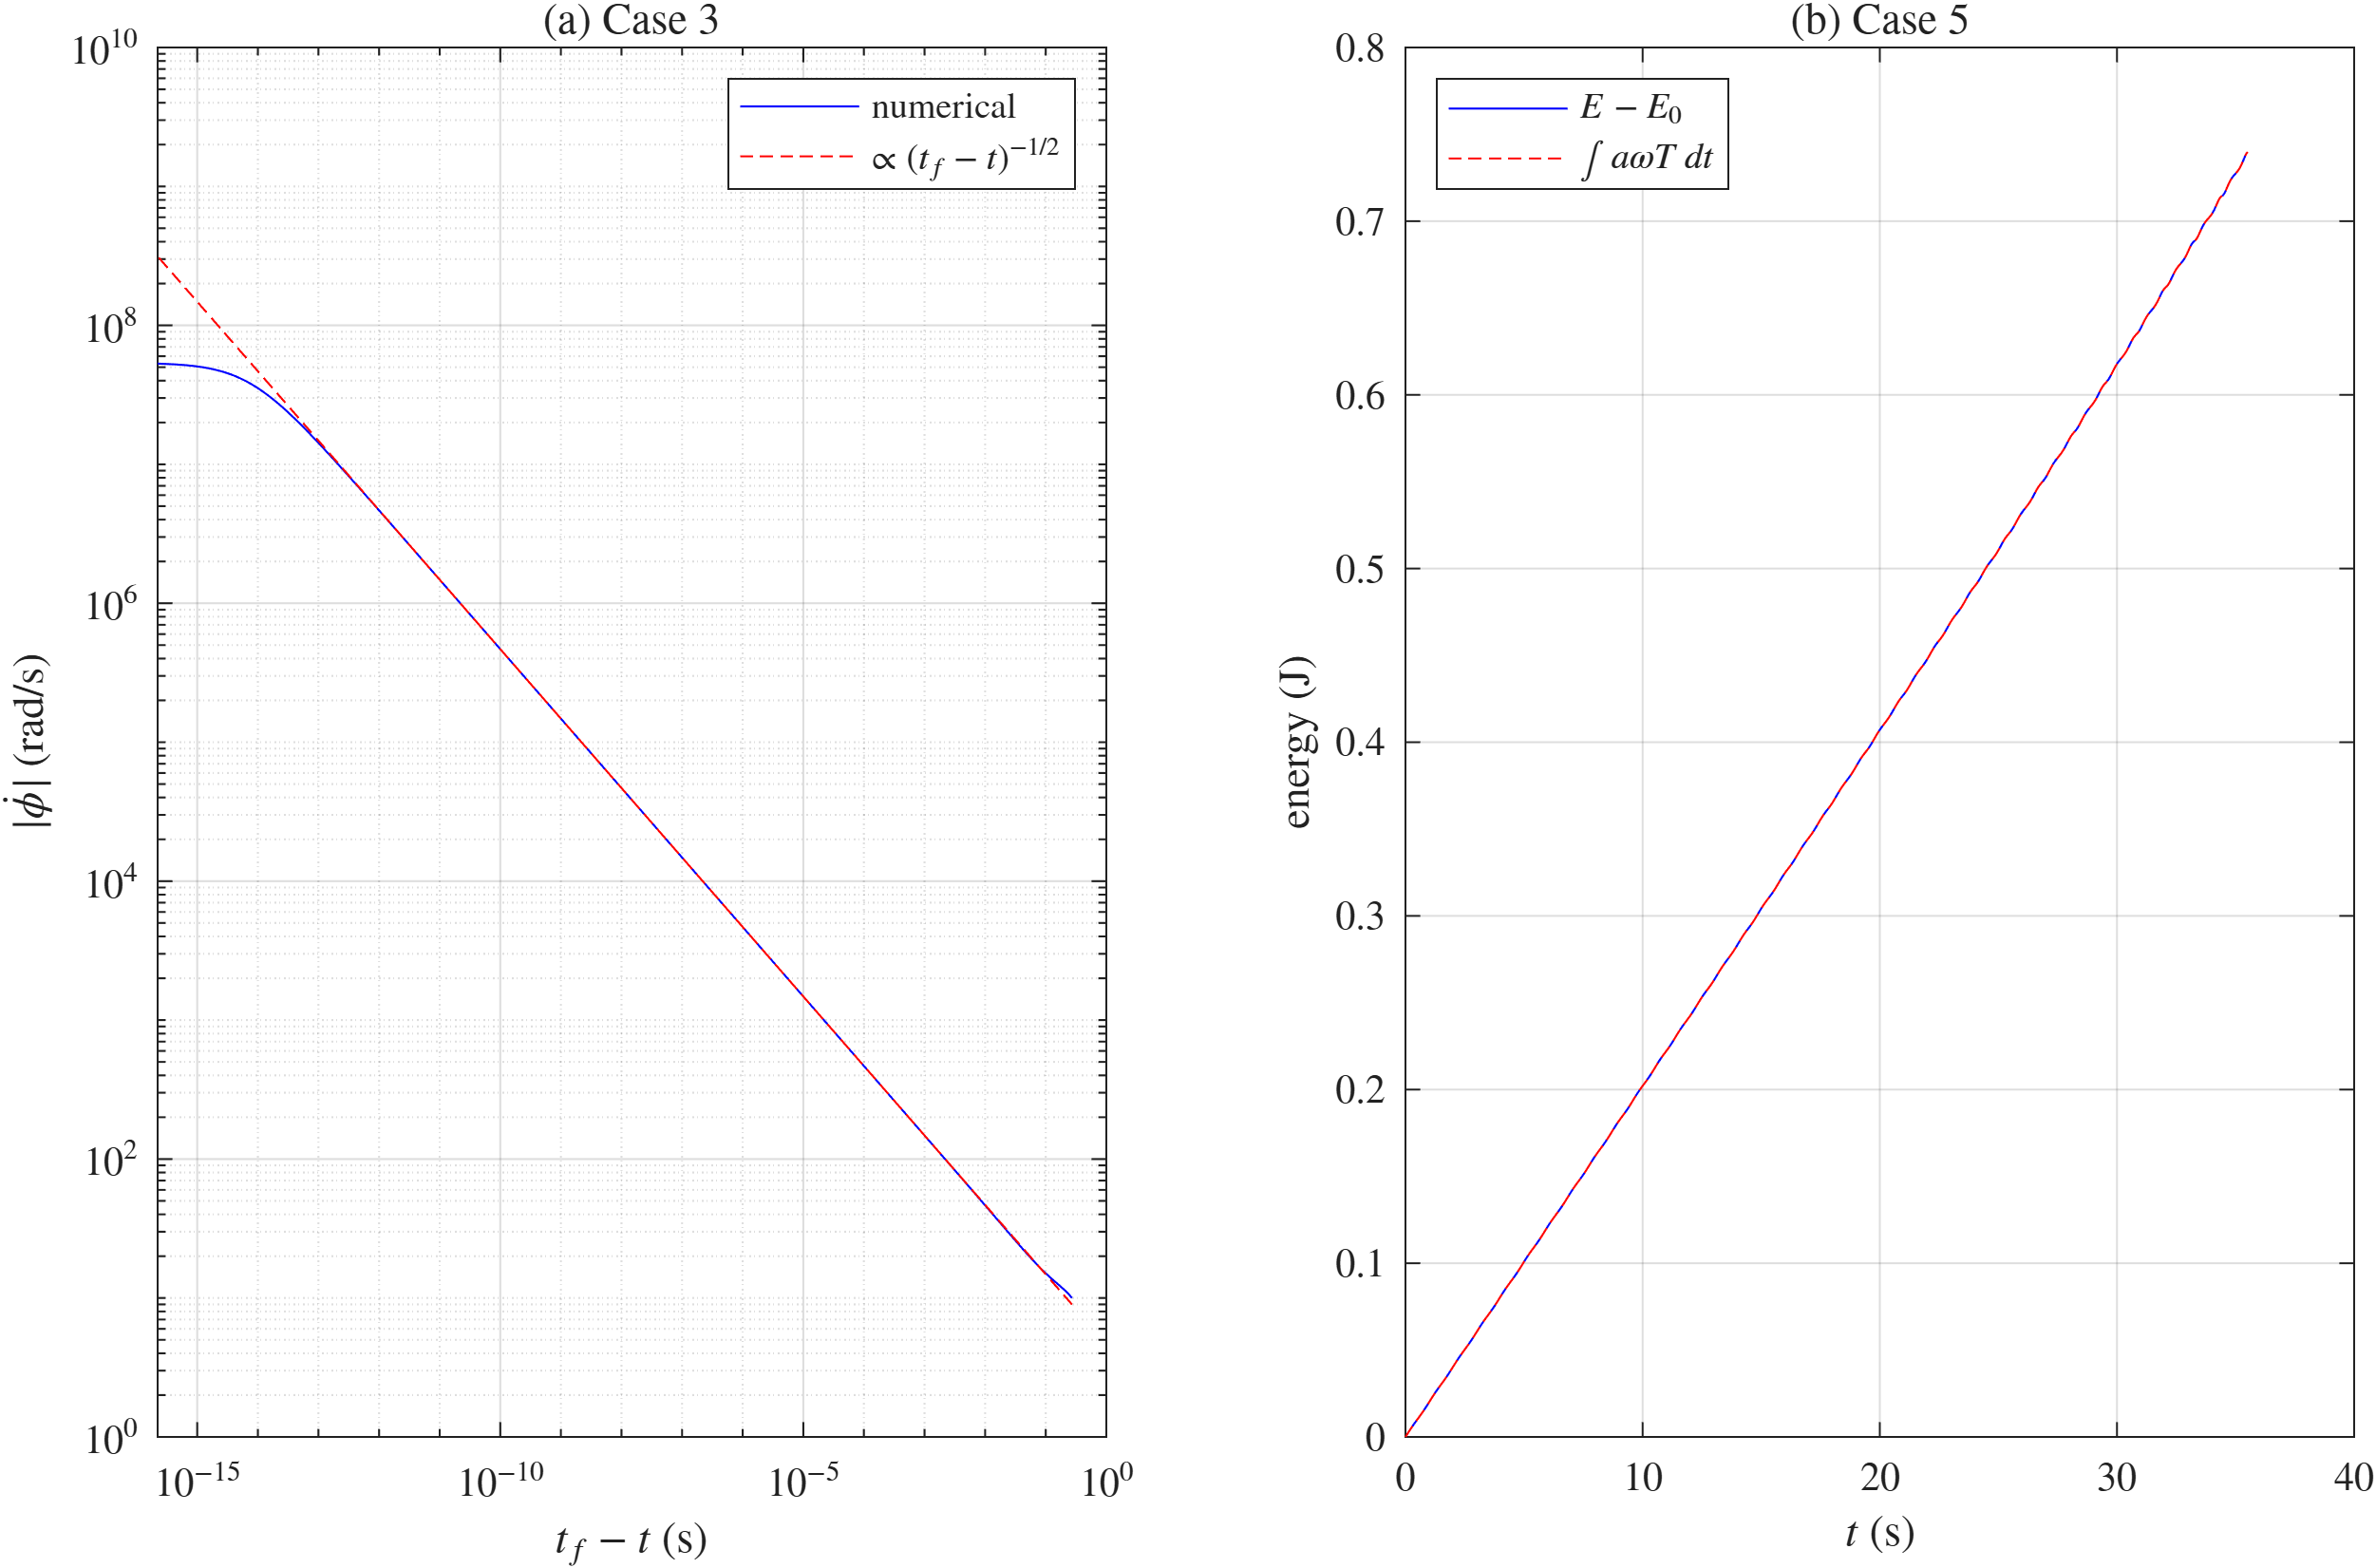
\includegraphics[width=0.62\textwidth]{Fig_4.png}
\caption{(a) Angular velocity of Case 3 as a function of the time remaining to the collision $t_f-t$, in logarithmic scale, together with the asymptotic law. (b) Work--energy check in Case 5: increment of mechanical energy and integral of the power $a\omega T$.}\label{fig:extra}
\end{figure}

\section{Conclusions}
The dynamics of a particle constrained by a winding string around a rotating cylinder was analyzed and solved numerically using \texttt{ode45}. Despite the continuous geometric winding, the system possesses a single degree of freedom parametrized by the angular position $\phi$, behaving as a generalized pendulum with time- and state-dependent length.

The mechanical energy balance governs the diverse responses observed across all five cases. When the spool is stationary ($\omega = 0$), the constraint forces perform no work, and mechanical energy is conserved within a relative numerical error below $10^{-9}$. Depending on the initial velocity, the motion manifests as bounded periodic oscillation (Case 2), rapid spiral winding leading to spool impact (Case 3), or string slackening upon deceleration above the spool (Case 4). Conversely, when the spool rotates ($\omega > 0$), work is continuously injected into the system at the rate $a\omega T$, lifting the particle at constant velocity (Case 1) or progressively amplifying the oscillation amplitude until spool impact occurs (Case 5). Numerical evaluation of the work integral using \texttt{ode45} verified the work-energy relation with high precision.

Finally, the operational boundaries of the single-degree-of-freedom formulation were identified. The mathematical model terminates under two distinct physical events: spool collision ($\xi \to 0$), where the angular velocity and tension exhibit power-law divergence $(t_f - t)^{-1/2}$, and loss of tension ($T = 0$), where the string ceases to support compressive forces. Beyond the slackening threshold, the particle uncouples from the spool constraint, requiring a two-degree-of-freedom ballistic model in Cartesian coordinates until tension is impulsively restored.


Therefore, we can say that the experiment successfully demonstrated the application of numerical integration to solve the equations of motion for a particle connected to a spool. The results provide insight into the dynamics of the system under varying initial conditions and angular velocities. Energy conservation was observed in cases where the string maintained tension, while the stop function correctly terminated the simulation when necessary. Future studies would be needed to focus on extending the analysis to the the cases where the string loses tension and the particle’s motion becomes unconstrained.

\begin{thebibliography}{9}
  \bibitem{guidelines}
  Aerospace Engineering Department (UC3M),
  \emph{Mechanics Applied to Aerospace Engineering: Laboratory Guidelines}, Version 2026.

  \bibitem{matlab}
  The MathWorks, Inc.,
  \emph{MATLAB Documentation: ode45, odeset}.
\end{thebibliography}

\end{document}
